\documentclass[11pt,a4paper]{ctexart}
\usepackage[margin=2.4cm]{geometry}
\usepackage{graphicx}
\usepackage{booktabs}
\usepackage{amsmath}
\usepackage{hyperref}

\title{超分辨下采样策略对 DFF 深度选择的影响}
\author{SRTP Project Notes}
\date{2026-06-21}

\begin{document}
\maketitle

\section{目的}

本报告进一步检查仿真采样策略是否会传导到传统 DFF 深度选择。实验比较两条路径：一是在高分辨率微几何上计算法线、眩光风险和焦堆，再下采样到传感器分辨率；二是直接在传感器分辨率上计算法线、眩光风险和焦堆。两者使用同一合成高度图作为 ground truth。

\section{结果}

\begin{table}[htbp]
\centering
\small
\begin{tabular}{rllrrrr}
\toprule
Factor & Mode & MAE & RMSE & P90 & High-risk MAE & Risk mean \\
\midrule
2 & superres & 0.0696 & 0.0827 & 0.1224 & 0.0804 & 0.0150 \\
2 & direct & 0.0688 & 0.0878 & 0.1216 & 0.0914 & 0.0216 \\
4 & superres & 0.0654 & 0.0759 & 0.1162 & 0.0686 & 0.0108 \\
4 & direct & 0.0717 & 0.0913 & 0.1247 & 0.0963 & 0.0254 \\
8 & superres & 0.0624 & 0.0717 & 0.1118 & 0.0624 & 0.0062 \\
8 & direct & 0.0748 & 0.0989 & 0.1272 & 0.1057 & 0.0288 \\
\bottomrule
\end{tabular}
\caption{DFF depth error under different simulation sampling strategies. Errors are normalized by the synthetic height range.}
\end{table}

\begin{figure}[htbp]
\centering
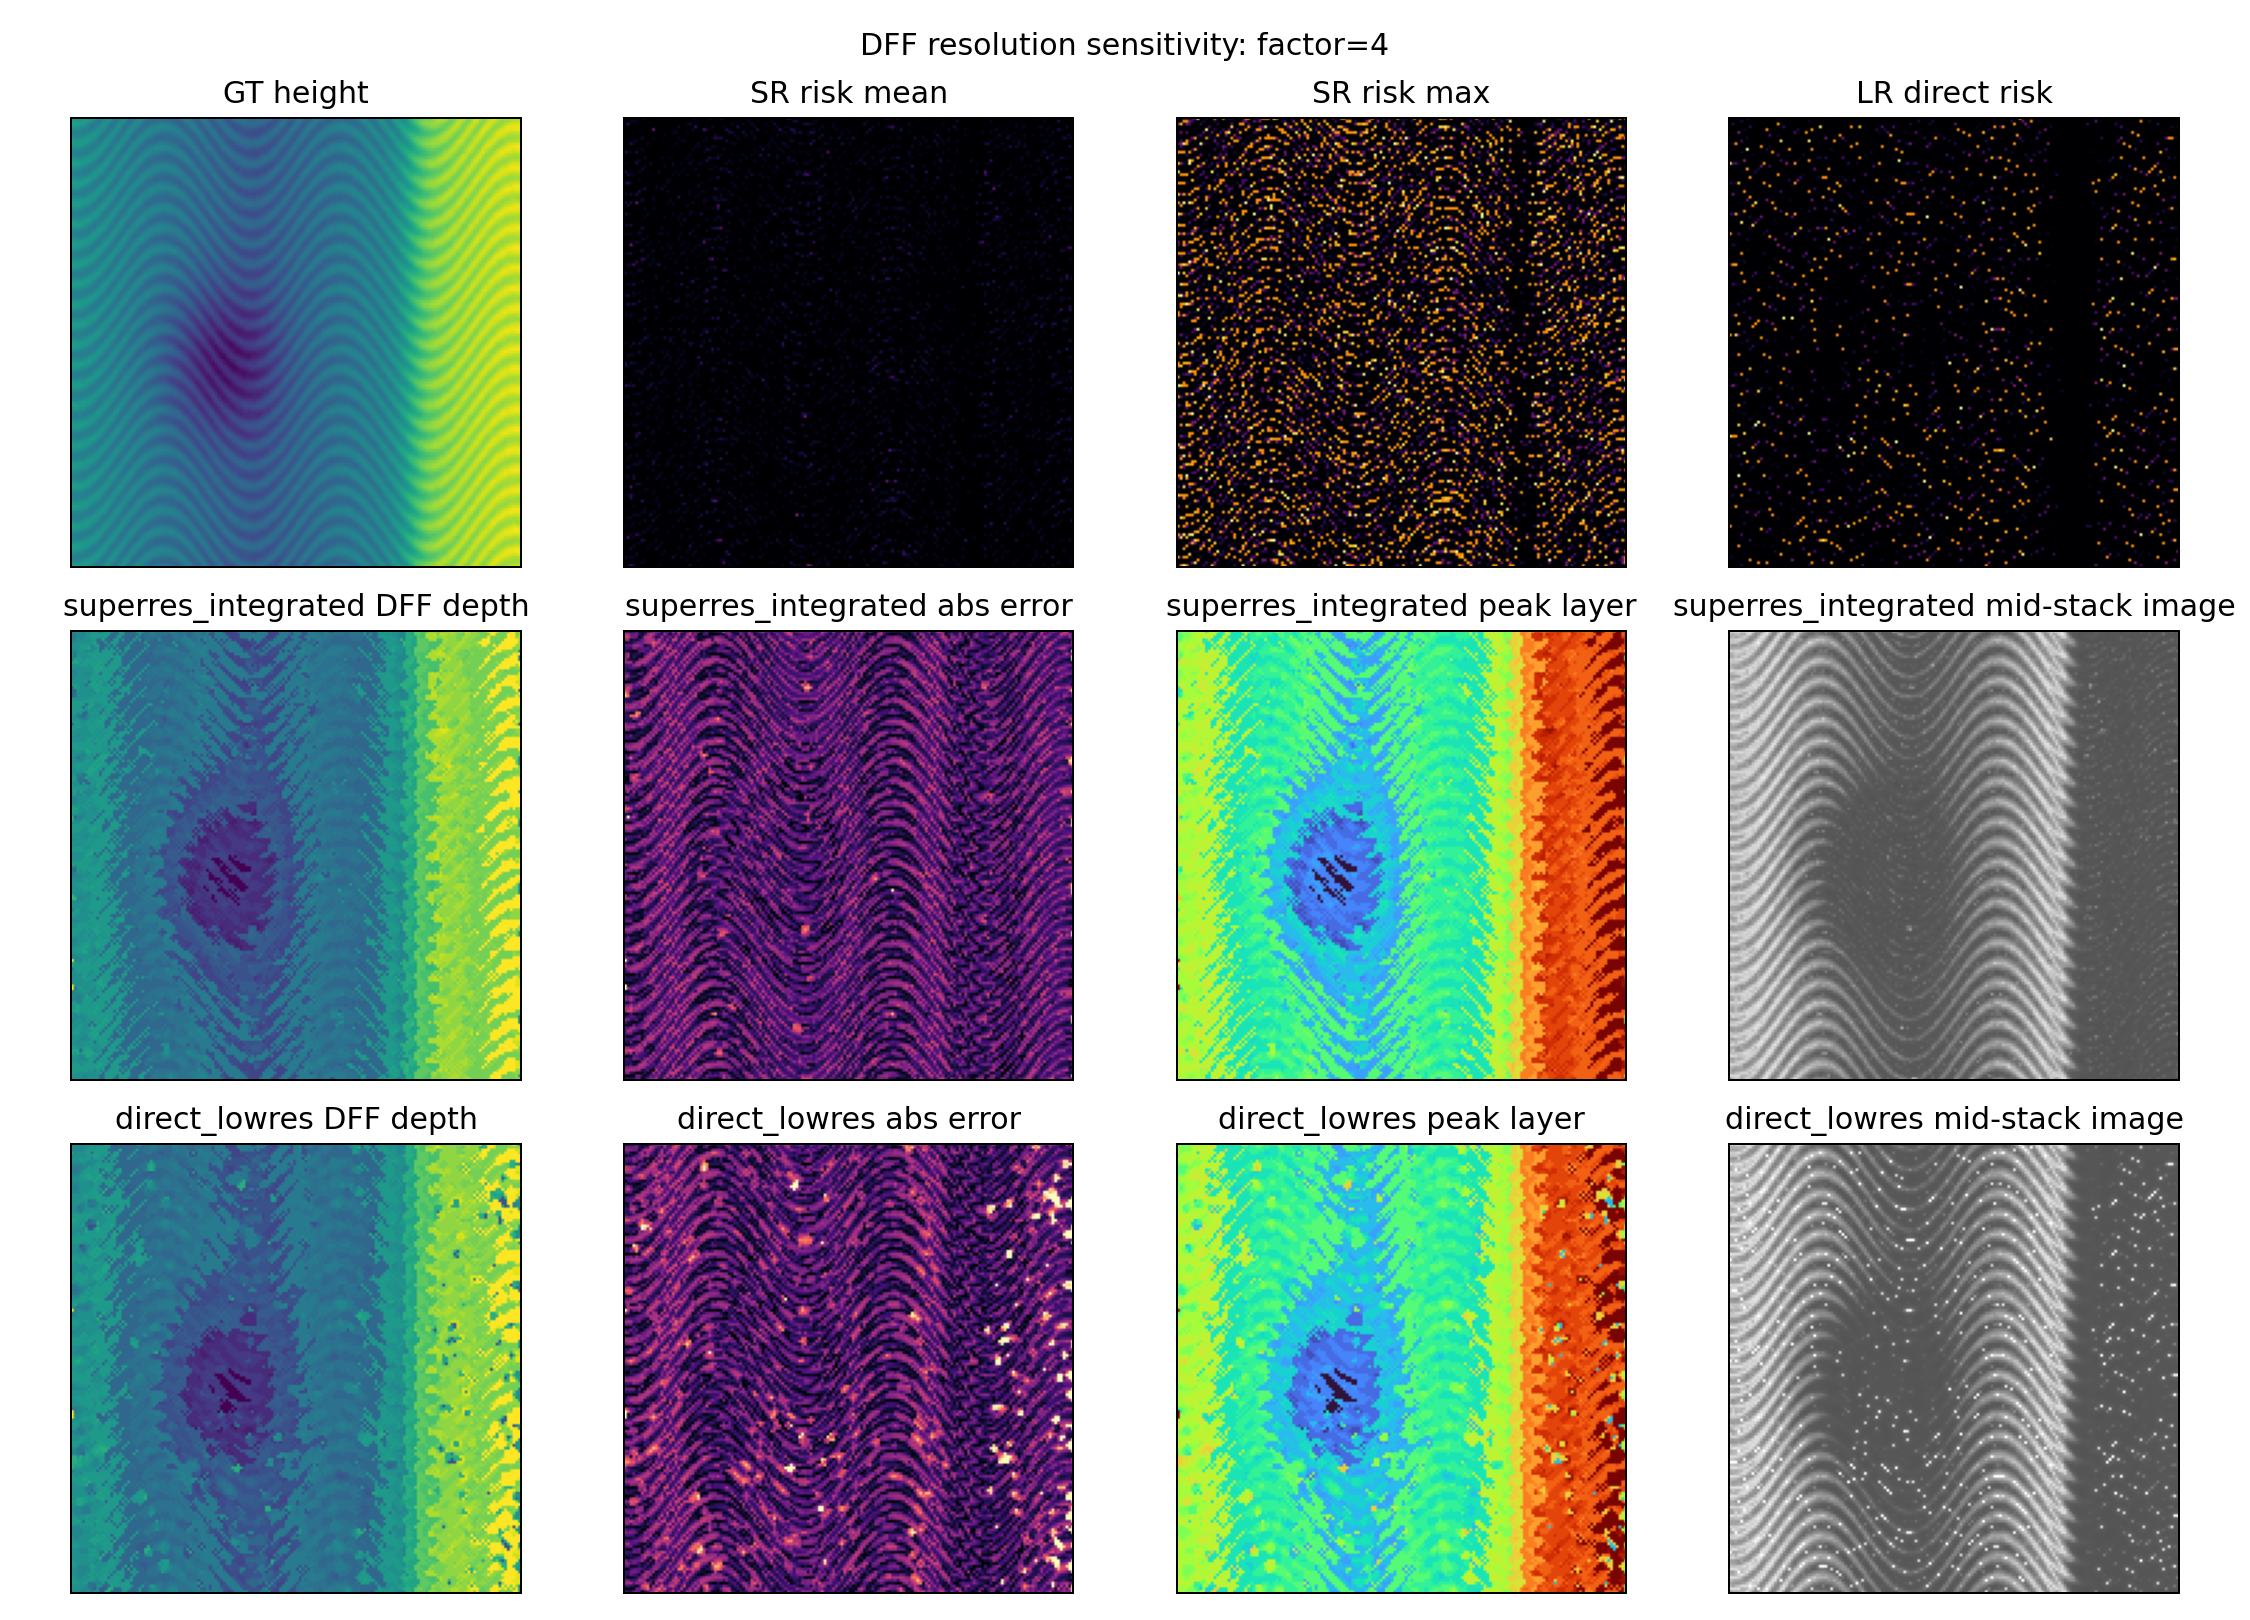
\includegraphics[width=0.95\linewidth]{dff_resolution_study/dff_factor_4_depth_error_panel.png}
\caption{DFF depth and error maps for 4x super-resolution integration versus direct low-resolution simulation.}
\end{figure}

\begin{figure}[htbp]
\centering
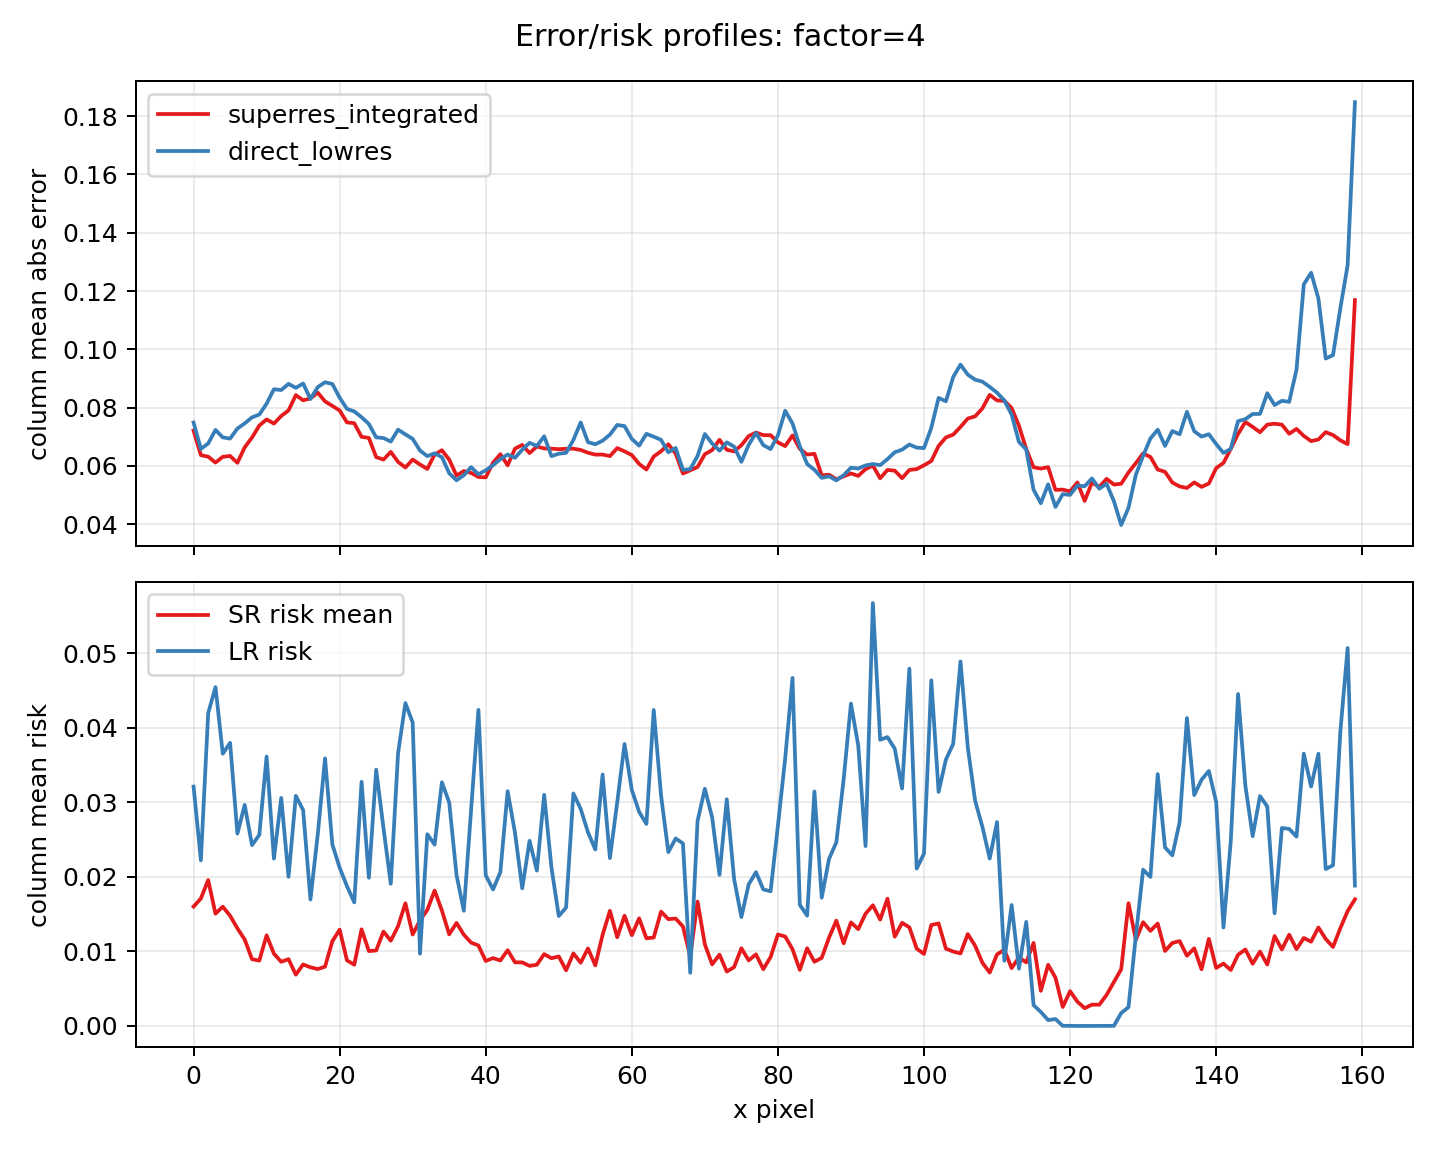
\includegraphics[width=0.95\linewidth]{dff_resolution_study/dff_factor_4_error_risk_profile.png}
\caption{Column-wise error and glare-risk profiles. Direct low-resolution simulation produces noisier risk profiles and higher edge-side error spikes.}
\end{figure}

\section{讨论}

结果显示，采样策略会影响 DFF 深度选择。4x 和 8x 设置下，\texttt{superres\_integrated} 的 MAE、RMSE、P90 error 和 high-risk MAE 均低于 \texttt{direct\_lowres}。8x 时，高风险区域误差从 0.0624 上升到 0.1057，说明直接低分辨法线估计对反光区域尤其敏感。

该结果支持一个新的方法设计原则：反光焦堆仿真应先在高分辨率微几何上计算法线、反射、离焦和曝光，再通过像素面积积分下采样到相机分辨率。该流程可以减少由数值网格引入的伪高亮和错误 focus response。

\section{论文可用表述}

\begin{quote}
To reduce grid-dependent artifacts in reflective simulation, the synthetic surface height, normal field, and glare-risk map are generated on a microgeometry grid higher than the target sensor resolution. Defocus, exposure clipping, and local reflectance are simulated in this high-resolution domain before the focal stack is integrated to the sensor resolution by block averaging or a pixel-aperture kernel.
\end{quote}

\section{结论}

本轮结果说明，超分辨下采样策略不只影响合成图像外观，也会影响传统 DFF 的深度选择和高风险区域误差。后续 synthetic generator 和消融实验应将 sampling-aware simulation 作为默认设计。

\end{document}
